% Paper template for TAR 2021
% (C) 2014 Jan Šnajder, Goran Glavaš, Domagoj Alagić, Mladen Karan
% TakeLab, FER

\documentclass[10pt, a4paper]{article}

\usepackage{tar2021}

\usepackage[utf8]{inputenc}
\usepackage[pdftex]{graphicx}
\usepackage{booktabs}
\usepackage{amsmath}
\usepackage{amssymb}
\usepackage{float}


\title{Syntax vs Semantics: What tells more about your personality?}

\name{Marko Lazarić, Laura Torić, Roman Yatsukha}

\address{
University of Zagreb, Faculty of Electrical Engineering and Computing\\
Unska 3, 10000 Zagreb, Croatia\\
\texttt{\{marko.lazaric,laura.toric,roman.yatsukha\}@fer.hr}\\
}

\abstract{
	Personality traits are inherently subjective and hard to define categories, so classifying peoples' personalities is a challenging task even for people.
	On the other hand, natural language processing has made great progress in similarly subjective areas such as sentiment analysis.
	In this paper, we compare two approaches to classifying individual personality traits based on essays: syntactic and semantic.
	The syntactic approach uses the role of the word in the sentence, such as subject, object, verb, etc., while the semantic approach uses the meaning of the words themselves to classify the essays.
	We compare the two approaches on a dataset of 2467 student essays annotated with the big five personality traits and show that the semantic approach tends to perform better across the board.
}

\begin{document}

\maketitleabstract

\section{Introduction}

Every text contains a remarkable amount of information about the author.
While that information might not be apparent to people, natural language processing has shown itself very adept at using that information to classify texts and their authors into certain categories.

An example of such a task is classifying the personality of the author based on their essay.
Since a personality is hard-to-define, it is usually decomposed into several personality traits which are usually binary.
The big five personality model is a popular personality trait model which will be used in this paper.
It uses the following five personality traits: extraversion, agreeableness, openness, conscientiousness and neuroticism.

In this paper, we experiment with two approaches to classifying the different personality traits: syntactic and semantic.
The syntactic approach uses the role of the words in the sentence such as subject, object, etc. without knowing what the words mean.
The semantic approach uses the meanings of the words, either through pretrained embeddings or the bag of words model.
Our results show that semantic models tend to perform better than syntactic models for all personality traits.
%Motivation (What we write tells alot about who we are.. bla bla ... how far can we go...)
%Big Five
%Previous work (only uses sentiment)
%But (what about the syntax?)
%We (will see what is more important syntax or semantics..)
%Results are showing..
%Overview

\section{Previous Work}

\citep{park} used five separate statistical models to predict personality traits of Facebook users, using their posts and self-reported Big5 personality traits.
They used both boolean encodings and relative frequencies of words and phrases, as well as topic extraction, as their features, which were then reduced using univariate feature selection, and randomized principal component analysis.
Although we use different features for our predictions, we mirror the idea of using separate models for each personality trait rather than predicting them with a single model.

In contrast, \citep{pizzolli-strapparava-2019-personality} used a single model on \citep{pennebaker} dataset with subpar results, although they used the essay dataset only for the purpose of having a baseline, before moving on to predict traits of various characters in William Shakespeare's Hamlet.

\section{Dataset}
%About dataset
%POS, NE, embeddings, bag of words

The dataset used for this paper is from \citep{pennebaker}, a collection of student essays.
The students' personality traits were assessed using the big five inventory (BFI) self-report questionnaire.
The dataset contains 2467  essays with a mostly balanced number of positive and negative examples for each class which is shown in table \ref{positive negative examples}.

\begin{table}[H]
	\centering
	\caption{The number of positive and negative examples for each personality trait.}
	\begin{tabular}{lrr}
		\toprule
		Personality trait & Negative & Positive \\ \midrule
		Extraversion                                  & 1191 (48.28\%)                         & 1276 (51.72\%)                         \\
		Neuroticism                                  & 1234 (50.02\%)                         & 1233 (49.98\%)                         \\
		Agreeableness                                  & 1157 (46.90\%)                         & 1310 (53.10\%)                         \\
		Conscientiousness                                  & 1214 (49.21\%)                         & 1253 (50.79\%)                         \\
		Openness                                  & 1196 (48.48\%)                         & 1271 (51.52\%)                         \\ \bottomrule
	\end{tabular}
	\label{positive negative examples}
\end{table}

Our goal is to correctly classify all of the big five personality traits based on the given essay.

\section{Features}

The features extracted from the essays were bag-of-words features and the number of each part-of-speech and named entity tag in the essay.
SpaCy\footnote{https://spacy.io} was used for lemmatization, part-of-speech tagging and named entity recognition.

To reduce the effect of the length of the essay on the features, alternative features were tried where each number was normalized by the sum of the part-of-speech or named entity tags to get the percentage of each tag or normalized by the number of sentences to get the mean number of each part-of-speech or named entity tag per sentence.

The previously explained features are shown in table \ref{example features} for the sentence "Well, right now I just woke up from a mid-day nap in Texas."
SpaCy's abbreviations for individual tags are used to preserve space.

\begin{table}[H]
	\centering
	\caption{Number of each part-of-speech and named entity tag detected by spaCy in the example sentence.}
	\begin{tabular}{llllll}
		\toprule
		\multicolumn{4}{l}{Part-of-speech tags} & \multicolumn{2}{l}{Named entity tags} \\ \midrule
		RB        & 3       & VBD      & 1      & DATE                & 1               \\
		NN        & 3       & RP       & 1      & GPE                 & 1               \\ \cline{5-6} 
		IN        & 2       & DT       & 1      &                     &                 \\
		UH        & 1       & JJ       & 1      &                     &                 \\
		,         & 1       & NNP      & 1      &                     &                 \\
		PRP       & 1       & .        & 1      &                     &                 \\ \cline{1-4}
	\end{tabular}
	\label{example features}
\end{table}

For the semantic models, we used word embeddings.

\section{Models}
%SVM, decision trees, BERT, XLNet

Since the different personality traits are independent, a separate model was trained to classify each personality trait.
To test the predictive power of syntactic features, SVMs were used, and XLNet was used as a representative semantic model.
The individual models and their pipelines are further explained in the following subsections.

\subsection{SVM}

Support Vector Machines from scikit-learn\footnote{https://scikit-learn.org/} were trained to classify the essays for each personality trait.
Feature selection was done by selecting a certain number of features with the highest ANOVA F-value.
After that, the selected features were standardized by subtracting the mean and scaling to unit variance and used to train the SVMs.

\subsection{XLNet}

XLNet is an auto-regressive language model introduced in \citep{DBLP:journals/corr/abs-1906-08237}.
It uses transformers with recurrence to output the joint probability of a sequence of tokens.
To calculate the probability, it uses all permutations of word tokens in a sentence, instead of just those to the left or right of the target token.

In this paper, we used a pretrained XLNet for sequence classification with the XLNet tokenizer from the transformers\footnote{https://huggingface.co/transformers/} package.
The tokenizer takes the raw text and limits the input to 500 tokens so any essays longer than that are trimmed (about 70\% of essays end up being trimmed).
The network was trained for 5 epochs with a batch size of 5.
Adam with the learning rate of $10^{-5}$ and $10^{-2}$ regularization was used to update the parameters.

\section{Experiments}
To test our syntax and semantic models we conducted three experiments described in this section.

\textbf{Experiment 1.} To test the performance of different models and features we decided to compare F1 and accuracy scores measured on the test set.
For the syntax models, we used SVM with all possible combinations of part-of-speech and named entity tags and tested all of them.
For the semantic models, we used XLNet and SVM with bag-of-words features.

\textbf{Experiment 2.}  In order to test if some personality traits had different distributions of part-of-speech or named entity tags than others, we used a t-test, or more accurately, Welch's t-test.
For a few selected most promising tags we tested the difference between every pair of traits and reported p values.
If the p value was less than 0.05 the difference was considered significant.

\textbf{Experiment 3.} For our last experiment, we wanted to find the most descriptive features for each trait using a univariate f test.

\section{Results}

\subsection{Experiment 1.}
The accuracy and F1 results of all the models and feature combinations are shown in table \ref{table:acc-f1}.
Summary of the model and features with the highest accuracy are shown in table \ref{table:best}.
In the tables we use the following abbreviations: Agreeableness==A, Conscientiousness==C, Extraversion==E, Neuroticism==N, Openness=O.

\begin{table*}
  \caption{The accuracy and F1 scores for all models and feature combinations (s: simple, d: detailed, nn: non-normalized, nbs: normalized by sum, nbsc: normalized by sentence count).}
  \begin{center}
  \begin{tabular}{lrrrrrrrrrr}
    \toprule
    Model and features  &  E acc         & N acc          & A acc          & C acc          &  O acc         & E F1           & N F1           & A F1           & C F1           & O F1\\
    \midrule
          Bag of words & 0.536          & 0.539          & 0.507          & \textbf{0.589} & 0.594          & 0.592          & 0.455          & 0.598          & 0.570          &  \textbf{0.645}\\
           PoS (s, nn) & 0.539          & 0.513          & 0.523          & 0.515          & 0.567          & 0.625          & 0.462          & 0.641          & 0.558          &  0.575\\
           PoS (d, nn) & 0.538          & 0.529          & 0.515          & 0.507          & 0.554          & 0.614          & 0.474          & 0.639          & 0.518          &  0.518\\
               NE (nn) & 0.538          & 0.502          & 0.505          & 0.528          & 0.549          & 0.624          & 0.518          & \textbf{0.644} & 0.541          &  0.618\\
      PoS + NE (s, nn) & 0.555          & 0.495          & 0.491          & 0.531          & \textbf{0.606} & 0.642          & 0.461          & 0.619          & 0.544          &  0.644\\
      PoS + NE (d, nn) & 0.521          & 0.529          & \textbf{0.523} & 0.567          & 0.570          & 0.608          & 0.474          & 0.633          & \textbf{0.588} &  0.557\\
          PoS (s, nbs) & 0.546          & 0.497          & 0.529          & 0.539          & 0.567          & 0.593          & 0.498          & 0.643          & \textbf{0.606} &  0.611\\
          PoS (d, nbs) & 0.551          & 0.523          & 0.512          & 0.487          & 0.560          & 0.632          & 0.533          & 0.576          & 0.540          &  0.557\\
              NE (nbs) & 0.536          & 0.512          & 0.505          & 0.560          & 0.547          & 0.632          & 0.518          & 0.610          & 0.573          &  0.610\\
     PoS + NE (s, nbs) & 0.565          & 0.507          & 0.500          & 0.552          & 0.560          & \textbf{0.633} & 0.464          & 0.614          & 0.576          &  0.597\\
     PoS + NE (d, nbs) & \textbf{0.570} & \textbf{0.534} & 0.500          & 0.549          & 0.576          & \textbf{0.635} & 0.528          & 0.600          & 0.593          &  0.591\\
         PoS (s, nbsc) & 0.555          & 0.525          & 0.504          & 0.497          & 0.565          & 0.610          & 0.551          & 0.633          & 0.535          &  0.623\\
         PoS (d, nbsc) & 0.539          & 0.531          & 0.505          & 0.534          & 0.536          & 0.553          & \textbf{0.553} & 0.607          & 0.553          &  0.551\\
             NE (nbsc) & 0.557          & 0.502          & 0.504          & 0.549          & 0.554          & 0.618          & 0.532          & 0.616          & 0.551          &  0.625\\
    PoS + NE (s, nbsc) & 0.568          & 0.504          & 0.513          & 0.551          & 0.593          & 0.631          & 0.533          & 0.619          & 0.585          &  \textbf{0.649}\\
    PoS + NE (d, nbsc) & 0.541          & 0.536          & 0.510          & 0.560          & 0.581          & 0.573          & \textbf{0.569} & 0.600          & 0.577          &  0.616\\
                 XLNet & \textbf{0.604} & \textbf{0.556} & \textbf{0.542} & \textbf{0.586} & \textbf{0.636} & 0.613          & 0.468          & \textbf{0.683} & 0.576          &  0.488\\
    \bottomrule
  \end{tabular}
  \end{center}
  \label{table:acc-f1}
\end{table*}

\begin{table}[H]
  \centering
  \caption{The F1 and accuracy scores for the best models and feature combinations.}
  \begin{tabular}{llrr}
    \toprule
    Trait & Model and features &     F1 & Accuracy \\
    \midrule
    E &   XLNet + embeddings &  0.613 &  0.604 \\
    N &   XLNet + embeddings &  0.468 &  0.556 \\
    A &   XLNet + embeddings &  0.683 &  0.542 \\
    C &   SVM + Bag of words &  0.570 &  0.589 \\
    O &   XLNet + embeddings &  0.488 &  0.636 \\
    \bottomrule
  \end{tabular}
  \label{table:best}
\end{table}

As can be seen from the tables, all models perform similarly, but semantic models perform just slightly better on all traits.

\subsection{Experiment 2.}

Results of t tests can be seen in table \ref{table:ttest}.
Only significant p values are reported.
It is interesting to notice that Neurotic and Openness traits are significantly different from Extrovert and Agreeable traits, but are not significantly different from each other.
This would suggest similar syntax styles between those two groups of personality traits, but more research is needed to confirm that.

\begin{table}[H]
  \centering
  \caption{P value for t test on part-of-speech tags which are significant.}
  \begin{tabular}{lrc}
    \toprule
    Traits & p value & PoS tag \\
    \midrule
    N vs A & 0.0119 & verb \\
    N vs A & 0.0115 & pronoun \\
    E vs O & 0.0141 & noun \\
    A vs O & 0.0044 & noun \\
    E vs N & 0.0020 & punctuation \\
    E vs O & 0.0034 & punctuation \\
    A vs O & 0.0154 & punctuation \\
    \bottomrule
  \end{tabular}
  \label{table:ttest}
\end{table}

\subsection{Experiment 3.}

Using word clouds we visualized the results of experiment 3.
Other than being amusing, the figures are quite different from each other which shows a lot of potential for good classification models.

\begin{figure}
\begin{center}
  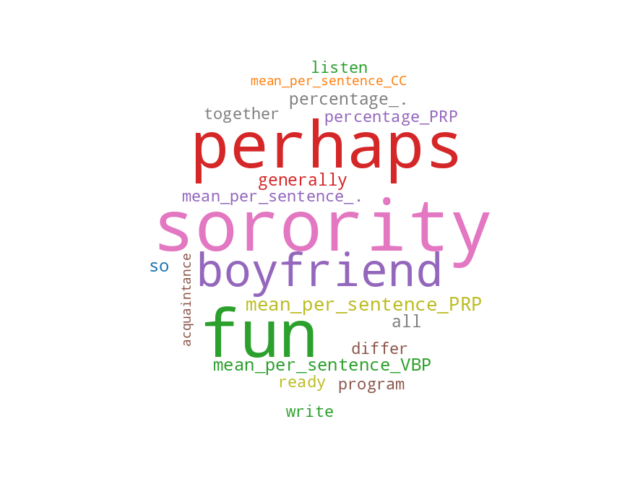
\includegraphics[width=\columnwidth]{figures/cEXT.png}
  \caption{Most significant features for the Extraversion trait.}
  \label{fig:figure1}
\end{center}
\end{figure}

\begin{figure}
\begin{center}
  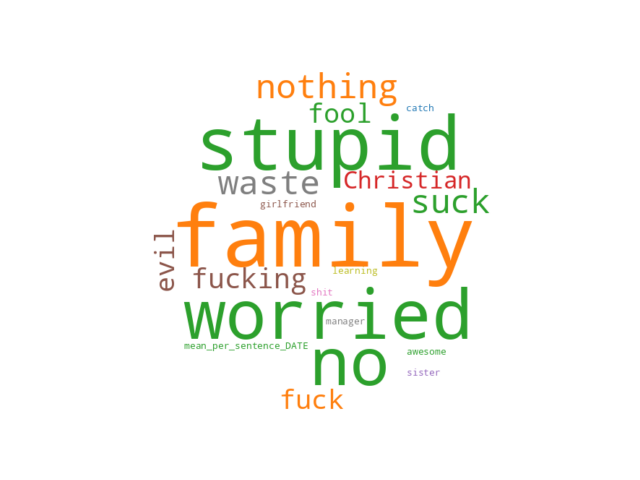
\includegraphics[width=\columnwidth]{figures/cAGR.png}
  \caption{Most significant features for the Agreeableness trait.}
  \label{fig:figure2}
\end{center}
\end{figure}

\begin{figure}
\begin{center}
  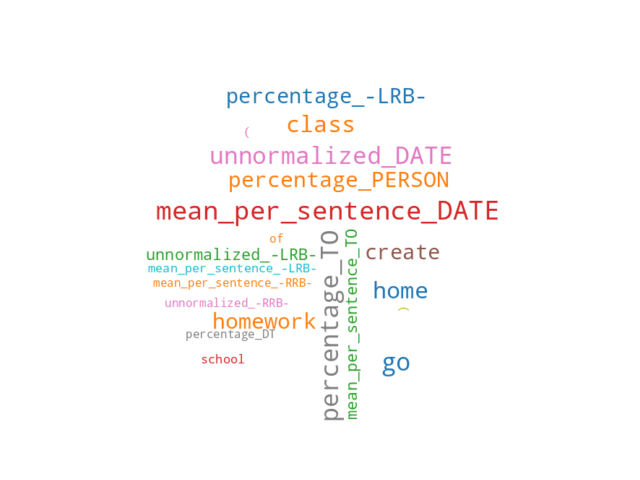
\includegraphics[width=\columnwidth]{figures/cOPN.png}
  \caption{Most significant features for the Openness trait.}
  \label{fig:figure3}
\end{center}
\end{figure}

\begin{figure}
\begin{center}
  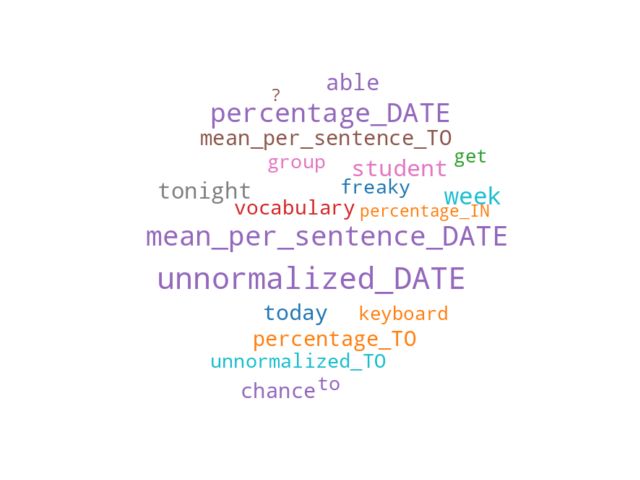
\includegraphics[width=\columnwidth]{figures/cCON.png}
  \caption{Most significant features for the Conscientiousness trait.}
  \label{fig:figure4}
\end{center}
\end{figure}

\begin{figure}
\begin{center}
  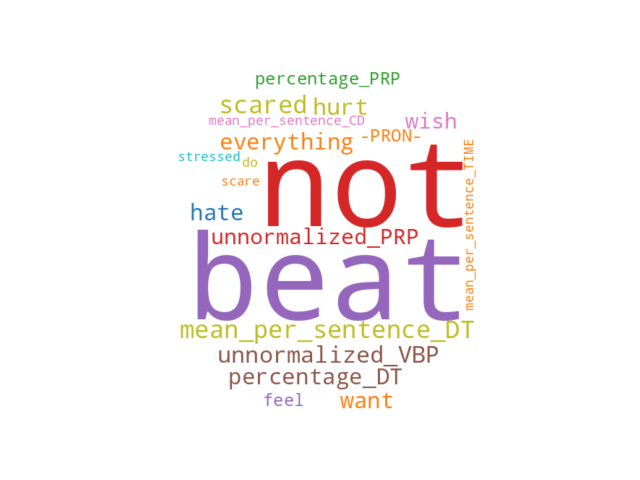
\includegraphics[width=\columnwidth]{figures/cNEU.png}
  \caption{Most significant features for the Neurotic trait.}
  \label{fig:figure5}
\end{center}
\end{figure}

\section{Conclusion}
In this paper, we compared only syntax and only semantic models to see if one has an edge over the other.
While there is certainly some information hiding in the syntax, semantics still seems to be the dominating factor.
By looking at the most important features for each personality, we can clearly see the differences between them, and some are not that surprising.
This promises a bright future for personality trait classification, and it seems that both syntax and semantics will be needed to create a powerful model.

\bibliographystyle{tar2021}
\bibliography{tar2021}

\end{document}
